% Created 2013-07-19 Fri 13:14
\documentclass[11pt]{article}
\usepackage[utf8]{inputenc}
\usepackage[T1]{fontenc}
\usepackage{graphicx}
\usepackage{longtable}
\usepackage{float}
\usepackage{wrapfig}
\usepackage{soul}
\usepackage{textcomp}
\usepackage{marvosym}
\usepackage{latexsym}
\usepackage{hyperref}
\tolerance=1000
\usepackage[italian]{babel}
\usepackage[usenames, dvipsnames]{xcolor}
\usepackage{minted}
\usepackage{amsmath}
\usepackage{amssymb}
\usepackage{amsthm}
\usepackage{amstext}
\usepackage{ulem}
\usepackage{makeidx}
\makeindex
\usepackage{accents} %serve per \underaccent, più bello di \underset
%\selectbiblanguage{italian}
\DeclareMathAlphabet{\mathpzc}{OT1}{pzc}{m}{it} %serve per \mathcpz
\numberwithin{equation}{subsection}

%altro
\newcommand{\defi}{\ensuremath{\stackrel{\mbox{\scriptsize{\textit{def}}}}{=}}}
\newcommand{\norm}[1]{\ensuremath{\left|\left|#1\right|\right|}}
\usepackage{algorithm}
\usepackage{algpseudocode}
\author{Renato Budinich}
\date{\today}
\title{Progetto per l'esame di Calcolo Scientifico}
\hypersetup{
  pdfkeywords={},
  pdfsubject={},
  pdfcreator={Emacs 24.3.1 (Org mode 8.0.5)}}
\begin{document}

\maketitle
\section{Descrizione del progetto}
\label{sec-1}
Il metodo di Lanczos, applicato ad una matrice hermitiana $A \in \mathbb{C}^{n\times n}$ con autovalori $\lambda_1\leq \ldots \leq \lambda_n$, fornisce al generico passo $k=1, \ldots, n$ una matrice tridiagonale $T_k \in \mathbb{C}^{k \times k}$ con autovalori $\mu_1^{(k)} \leq \ldots \leq \mu_k^{(k)}$. Gli autovalori estremi di $T_k$ convergono a quelli estremi di $A$, con velocità via via minore come ci si allontana dalle estremità ($\mu_{k-1}^{(k)}$ e $\mu_2^{(k)}$ convergono a $\lambda_{n-1}$ e $\lambda_2$ più lentamente di quanto $\mu_k^{(k)}$ e $\mu_1^{(k)}$ convergano a $\lambda_n$ e $\lambda_1$).

Lo scopo del progetto era verificare questa convergenza sulla matrice 

\begin{align*}
A \defi
\begin{bmatrix}
5 & 4 & 1 & & 0\\
4 & 6 & \ddots & \ddots & \\
1 & \ddots & \ddots & \ddots & 1\\
& \ddots & \ddots & 6 & 4  \\
0 & & 1 & 4 & 5
\end{bmatrix}
\end{align*}

che è il quadrato della matrice

\begin{align*}
\begin{bmatrix}
2 & 1 & & 0\\
1 & \ddots & \ddots & \\
& \ddots & \ddots & 1 \\
0 & & 1 & 2
\end{bmatrix}
\end{align*}

e della quale si conosce quindi l'espressione esplicita per gli autovalori

\begin{align}
\label{lambda}
\lambda_j = (2 + 2 \cos(\pi \frac{n+1-j}{n+1}))^2 \quad j=1,2, \ldots, n
\end{align}

che rende facile la verifica del metodo.
\section{L'algoritmo e l'implementazione}
\label{sec-2}
Il metodo di Lanczos fornisce delle relazioni ricorsive per gli autovettori $q_k, \, k=1, \ldots, n$ di $A$, per il vettore diagonale e per quello sopradiagonale (rispettivamente $\alpha$ e $\beta$) di $T_n$:

\begin{align}
\label{relaz}
\left\{
\begin{array}{ll}
q_{k+1} &= \frac{Aq_k -\alpha_k q_k - \beta_{k-1}q_{k-1}}{\beta_k} \\
q_1 &= q \\
q_0 &= 0
\end{array}
\right.
\quad \left\{
\begin{array}{ll}
\alpha_k &= q_k \cdot A q_k \\
\beta_k &= \norm{Aq_k -\alpha_k q_k - \beta_{k-1}q_{k-1}}
\end{array}
\right.
k=1, \ldots, n
\end{align}
dove $q$ è un vettore qualunque di norma $1$, e nel caso $\beta_k$ sia uguale a $0$, per $q_{k+1}$ basta scegliere un vettore ortogonale a $q_1,\ldots, q_k$.
Gli autovalori della matrice 

\begin{align*}
T_n = \begin{bmatrix}
\alpha_1 & \beta_1 & & 0\\
\beta_1 & \ddots & \ddots & \\
& \ddots & \ddots & \beta_{n-1} \\
0 & & \beta_{n-1} & \alpha_n
\end{bmatrix}
\end{align*}

così ottenuta sono in teoria esattamente gli autovalori di $A$; in realtà a causa degli errori numerici saranno delle approssimazioni. Solitamente il metodo viene usato come metodo iterativo, sfruttando la proprietà di convergenza già accennata: ci si ferma all'iterazione $K$ e si usano gli autovalori estremi di $T_K$ come approssimazione di quelli di $A$.

\begin{algorithm} 
\caption{}
\label{algo}
\begin{algorithmic}
\State $q_0 \gets 0$
\State $q_1 \gets$ vettore random di norma $1$
\For{$k=1,\ldots,K$}
\State $t \gets A q_k$
\State $\alpha_k \gets q_k \cdot t$
\State $r \gets t - \alpha_k q_k - \beta_{k-1}q_{k-1}$
\If{$k<n$}
\State $\beta_{k} \gets \norm{r}$
\If{$\beta_k \neq 0$}
\State $q_{k+1} \gets \frac{r}{\beta_k}$
\Else 
\State break
\EndIf
\EndIf
\EndFor
\end{algorithmic}
\end{algorithm}

Dalle relazioni (\ref{relaz}) si ricava l'algoritmo (\ref{algo}), il cui costo dominante è la moltiplicazione matrice per vettore $A q_k$, che nel nostro caso, essendo $A$ pentadiagonale, ha complessità $\mathcal{O}(n)$; quindi l'algoritmo globalmente ha complessità temporale $\mathcal{O}(nK)$, dove $K$ è il numero di iterazioni effettuate.

La complessità in memoria dell'algoritmo è $\mathcal{O}(nK)$, perchè bisogna memorizzare la matrice $Q$ degli autovettori; siccome questi non interessavano, ho usato invece l'algoritmo (\ref{algo2}) che ha complessità in memoria $\mathcal{O}(K)$.

\begin{algorithm}[H]
\caption{}
\label{algo2}
\begin{algorithmic}
\State $w \gets 0$
\State $v \gets$ vettore random di norma $1$
\For{$k=1,\ldots,K$}
\State $t \gets A v$
\State $\alpha_k \gets v \cdot t$
\State $r \gets t - \alpha_k v - \beta_{k-1}w$
\If{$k<n$}
\State $\beta_{k} \gets \norm{r}$
\If{$\beta_k \neq 0$}
\State $z \gets \frac{r}{\beta_k}$
\State $w \gets v$
\State $v \gets z$
\Else 
\State break
\EndIf
\EndIf
\EndFor
\end{algorithmic}
\end{algorithm}

\subsection{Codice sorgente}
\label{sec-2-1}
Segue l'implementazione in Fortran dell'algoritmo. Ho usato la subroutine \href{http://www.netlib.org/lapack/explore-html/d9/d45/dstevr_8f.html#}{DSTEVR} di LAPACK per calcolare ad ogni passo gli autovalori di $T_k$. 

Nel codice ad ogni iterazione controllo se $|\beta(k)| \leq \epsilon$, costante fissata inizialmente, per evitare problemi di instabilità numerica; si veda ad esempio la figura (\ref{epsilon_piccolo}), dove $\epsilon$ è stato fissato abbastanza piccolo da non entrare mai nel ramo dell' \verb~if~ che interrompe il ciclo iterativo - vengono svolte quindi tutte le $K$ iterazioni, e si vede che da una certa iterazione in poi gli errori di alcuni autovalori più interni cominciano ad aumentare. Invece ponendo $\epsilon = 1$ l'iterazione si ferma prima di tale fenomeno (che ho riscontrato sperimentalmente in molte altre istanze) fornendo un'approssimazione migliore di quegli autovalori.

\begin{figure}[htb]
\centering
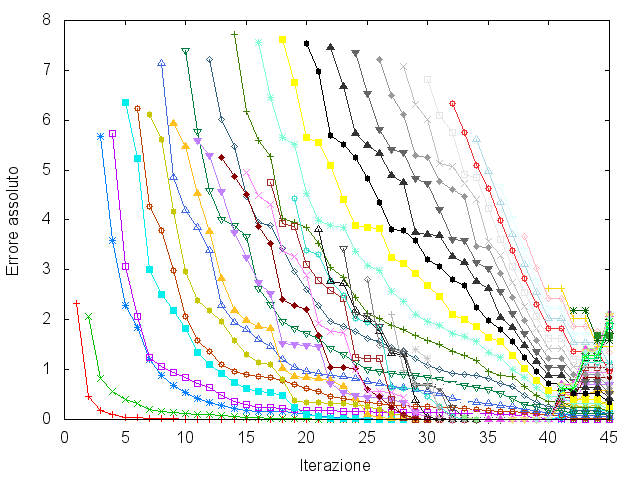
\includegraphics[width=.9\linewidth]{./img/errors_n45K45eps-3.png}
\caption{\label{epsilon_piccolo}Errori per $n=45, K=45, \epsilon=10^{-3}$}
\end{figure}

\begin{figure}[htb]
\centering
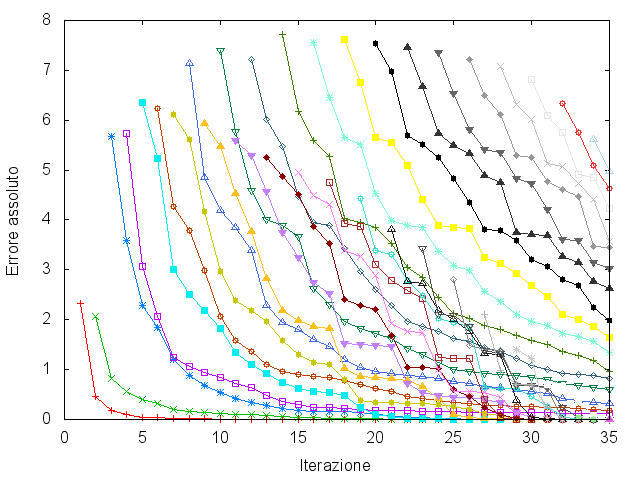
\includegraphics[width=.9\linewidth]{./img/errors_n45K45eps0.png}
\caption{\label{epsilon_grande}Errori per $n=45, K=45, \epsilon=1$}
\end{figure}

\begin{minted}[]{fortran}
PROGRAM lanczos
  IMPLICIT NONE
  INTEGER, PARAMETER :: dp=KIND(0.d0)
  INTEGER :: k,j, n, left_index, right_index, iterations, uscito = 0
  REAL(dp) :: epsilon =1.e0
  REAL(dp), DIMENSION(:), allocatable :: rnd, t, alfa, beta, r, &
       v, w, z, eig, alfa_tmp, beta_tmp

  WRITE(*,*) "Assegna la dimensione n della matrice A:"
  READ(*,*) n
  WRITE(*,*) "Assegna il numero di iterazioni K da effettuare"
  READ(*,*) iterations
  iterations = min(iterations,n)

  ALLOCATE(rnd(n),t(n),alfa(iterations),beta(iterations),r(n),&
       v(n),w(n),z(n),eig(iterations),alfa_tmp(n),beta_tmp(n))

  OPEN(unit=4, file="errors.txt")
  OPEN(unit=5, file="eigv.txt")
  OPEN(unit=6, file="correcteigv.txt")
  WRITE(6,*) "#Correct eigenvalues:"
  DO j=1,n
     WRITE(6,*) correctegv(j,n)
  END DO
  WRITE(5,*) "#Approximated eigenvalues"

  CALL random_seed
  CALL random_number(rnd)
  v = rnd/NORM2(rnd)
  w = 0
  DO k=1, iterations
     CALL prodotto(v, n, t)
     alfa(k) = dot_product(v, t)
     r = t - alfa(k)*v - beta(k-1)*w
     IF (k < n) then
	beta(k) = norm2(r)
	IF (abs(beta(k)) <= epsilon) then
	   WRITE(0,*) "|beta(k)| <= epsilon =", epsilon, " per k = ", k
	   uscito = 1
	   exit
	END IF
	z = r/beta(k)
     END IF
     w = v
     v = z

     !la seguente subroutine scrive in eig i k autovalori di T_k
     !siccome DSTEVR, la routine di LAPACK utilizzata, potrebbe moltiplicare
     !i vettori diagonali e sopradiagonali per evitare instabilita' numerica,
     !gliene passo delle copie per lasciare i vettori alfa e beta inalterati
     alfa_tmp = alfa
     beta_tmp = beta
     CALL eigenvalues(alfa_tmp(1:k), beta_tmp(1:k), eig, k)

     WRITE(5,"(I4 A)", advance = "no") k, " " 
     WRITE(4,"(I4 A)", advance = "no") k, " " 
     DO j=1, k
	IF (mod(j,2)==1) then
	   right_index = k - ceiling(REAL(j)/2.0) + 1
	   WRITE(4, "(F12.9 A)", advance="no") abs(correctegv(right_index + n -k,n)&
		- eig(right_index)), " "
	   WRITE(5,"(F12.9 A)", advance="no") eig(right_index), " "
	else
	   left_index = j/2
	   WRITE(4, "(F12.9 A)", advance="no") abs(correctegv(left_index,n)&
		- eig(left_index)), " "
	   WRITE(5, "(F12.9 A)", advance="no") eig(left_index), " "
	END IF
     END DO
     WRITE(5,*)
     WRITE(4,*)
  END DO

  IF (uscito == 1) then
     k = k + 1
  END IF

  WRITE(5,*) "#iterations: ", k - 1
  WRITE(4,*) "#iterations: ", k - 1
  WRITE(0,"(A I6 A)") "ho effettuato", k-1, " iterazioni, esco"

CONTAINS

  REAL FUNCTION correctegv(i,n)
    IMPLICIT NONE
    INTEGER :: i,n
    INTEGER, PARAMETER :: dp=KIND(0.d0)
    REAL(dp) :: pi = acos(-1.0)
    correctegv = (2+2* cos(pi *(REAL(n -i +1)/REAL((n+1)))))**2
    RETURN
  END FUNCTION correctegv

  SUBROUTINE prodotto(invec, n, outvec) !calcola outvec=A invec
    IMPLICIT NONE
    INTEGER, PARAMETER :: dp=KIND(0.d0)
    INTEGER :: n, i
    REAL(dp), DIMENSION(n) :: invec,outvec

    outvec(1) = 5*invec(1) + 4*invec(2) + invec(3)
    outvec(2) = 4*invec(1) + 6*invec(2) + 4*invec(3) + invec(4)
    DO i = 3, n-2
       outvec(i) = invec(i-2) + 4*invec(i-1) + 6*invec(i) + 4*invec(i+1) + invec(i+2)
    END DO
    outvec(n-1) = invec(n-3) + 4*invec(n-2) + 6*invec(n-1) + 4*invec(n)
    outvec(n) = invec(n-2) + 4*invec(n-1) + 5*invec(n)
    return
  END SUBROUTINE prodotto

  SUBROUTINE eigenvalues(d, u, eig, n)
    implicit none
    INTEGER :: n
    CHARACTER :: JOBZ = 'N', RANGE = 'A'
    !lower and upper bounds of wanted eigenvalues 
    !used only IF RANGE = 'V':
    REAL(dp) :: VL, VU 
    !lower and upper index (ascending order) of wanted eigenvalues
    !used only IF RANGE = 'I':
    INTEGER :: IL, IU 
    REAL(dp) :: ABSTOL = 1.e-5 !tolerance on approximation error of eigenvalues
    REAL(dp), dimension(n):: eig, d !array with eigenvalues, diagonal
    REAL(dp), dimension(n - 1):: u !upper diagonal
    REAL(dp), dimension(:), allocatable :: Z !not referenced IF JOBZ='N'
    INTEGER, dimension(2*n) :: ISUPPZ
    INTEGER :: LWORK, LIWORK
    REAL(dp), dimension(:), allocatable :: WORK
    INTEGER, dimension(:), allocatable :: IWORK
    INTEGER :: INFO, M

    ALLOCATE(WORK(1), IWORK(1))
    CALL DSTEVR(JOBZ, RANGE, n, d, u, VL, VU, IL, IU, ABSTOL, n, eig,Z, n,&
	 ISUPPZ,WORK, -1, IWORK, -1,INFO)
    LWORK = WORK(1)
    LIWORK = IWORK(1)
    DEALLOCATE(WORK, IWORK)
    ALLOCATE(WORK(LWORK), IWORK(LIWORK))
    CALL DSTEVR(JOBZ, RANGE, n, d, u, VL, VU,IL,IU,ABSTOL,M,eig,Z,n,&
	 ISUPPZ,WORK,LWORK,IWORK,LIWORK,INFO)
    DEALLOCATE(WORK, IWORK)
  END SUBROUTINE eigenvalues
END PROGRAM lanczos
\end{minted}
\section{Utilizzo del programma ed interpretazione dell'output}
\label{sec-3}
Il programma chiede in input $n$ ed il numero di iterazioni $K$ da effettuare, e fornisce in output tre file:

\begin{description}
\item[correcteigv.txt] contiene gli $n$ autovalori di $A$ in ordine crescente, uno per riga, calcolati usando la (\ref{lambda})
\item[eigv.txt] c'è una riga per ogni iterazione effettuata; la prima colonna è l'indice $k$ dell'iterazione, quelle successive sono gli autovalori di $T_k$, ordinati in questo modo: $\mu_k^{(k)}, \mu_1^{(k)}, \mu_{k-1}^{(k)}, \mu_2^{(k)}, \ldots$.
\item[errors.txt] anche qui la prima colonna è l'indice $k$ dell'iterazione, quelle successive invece sono le differenze in valore assoluto tra gli autovalori corretti e quelli approssimati, con lo stesso ordine del file precedente, ovvero: $|\lambda_n - \mu_k^{(k)}|, |\lambda_1 - \mu_1^{(k)}|, |\lambda_{n-1} - \mu_{k-1}^{(k)}|, |\lambda_2 - \mu_2^{(k)}|, \ldots$
\end{description}

Questi file vengono poi utilizzati dagli script \verb~gnuplot~ \verb~plot-eigv.gp~ e \verb~plot-err.gp~ per produrre dei grafici rispettivamente della convergenza e degli errori commessi, al crescere delle iterazioni. 

Per eseguire il programma e visualizzare il grafico degli errori si può ad esempio dare il comando:
\begin{minted}[]{bash}
$ gfortran lanczos.f90 -llapack -o lanczos && ./lanczos && gnuplot plot-err.gp
\end{minted}

Per il grafico della convergenza degli autovalori (che è utile solo per valori piccoli di $n$) basta sostituire \verb~plot-eigv.gp~ a \verb~plot-err.gp~ nel comando sopra. In questo grafico le linee rosse sono le rette $y = \lambda_j, j=1, \ldots, n$.

Nelle figure sono riportati alcuni esempi dei grafici prodotti per diversi valori di $n$ e $K$.

\begin{figure}[htb]
\centering
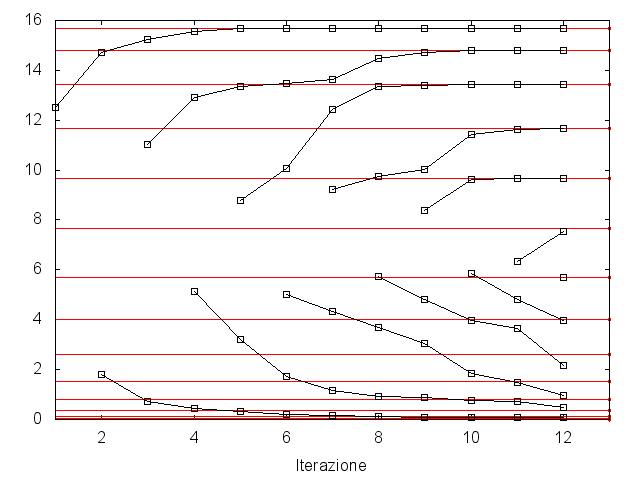
\includegraphics[scale=0.65]{img/eigv_n15K15.png}
\caption{Convergenza degli autovalori per $n = K = 15$}
\end{figure}

\begin{figure}[htb]
\centering
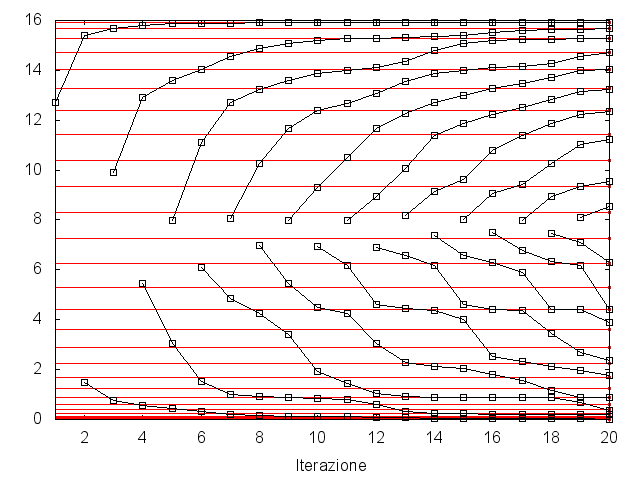
\includegraphics[scale=0.65]{img/eigv_n30K20.png}
\caption{Convergenza degli autovalori per $n = 30, K = 20$}
\end{figure}

\begin{figure}[htb]
\centering
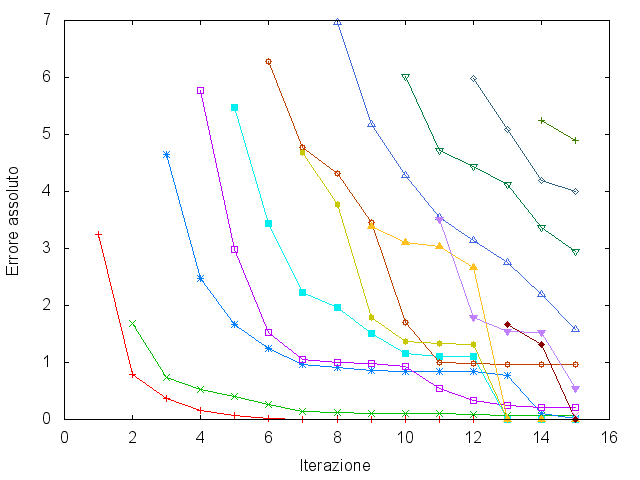
\includegraphics[scale=0.65]{./img/errors_n20K20.png}
\caption{Errori per $n=20, K=20$}
\end{figure}

\begin{figure}[htb]
\centering
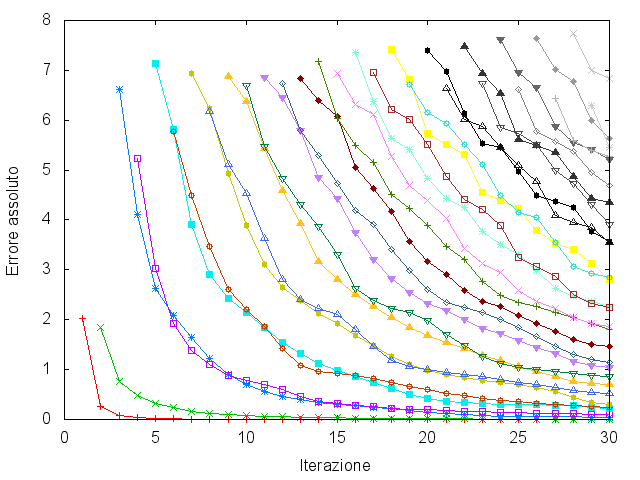
\includegraphics[scale=0.65]{./img/errors_n100K30.png}
\caption{Errori per $n=100, K=30$}
\end{figure}

\begin{figure}[htb]
\centering
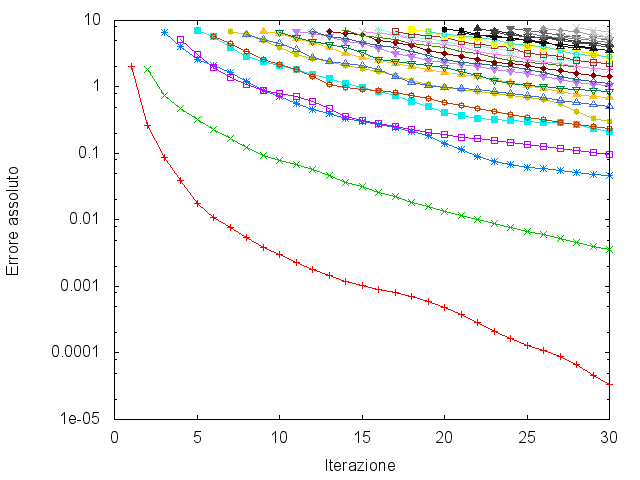
\includegraphics[scale=0.65]{./img/errors_n100K30_log.png}
\caption{Errori per $n=100, K=30$ in scala logaritmica}
\end{figure}

\begin{figure}[htb]
\centering
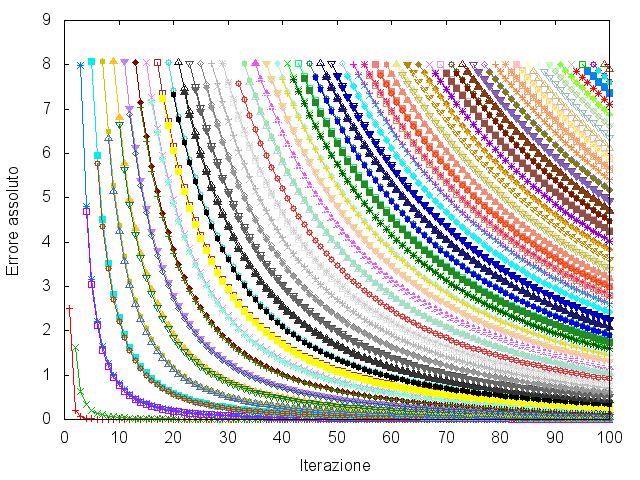
\includegraphics[scale=0.65]{./img/errors_n10^6K100.png}
\caption{\label{errori_ngrande}Errori per $n=10^6, K=100$}
\end{figure}

\begin{figure}[htb]
\centering
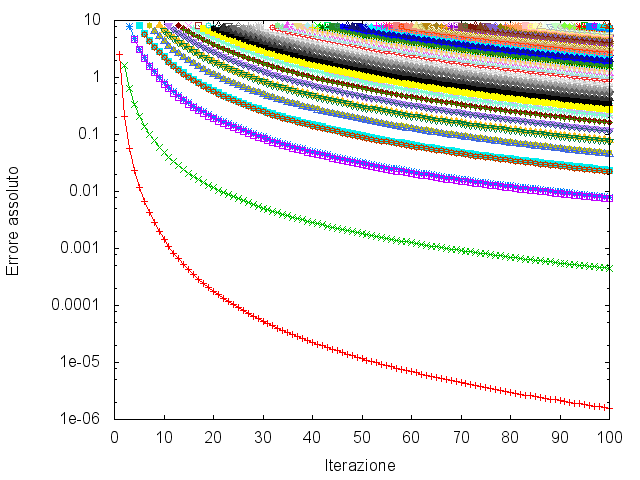
\includegraphics[scale=0.65]{./img/errors_n10^6K100_log.png}
\caption{Errori per $n=10^6, K=100$ in scala logaritmica}
\end{figure}


\section{Commenti}
\label{sec-4}
Dai grafici degli errori si nota come la convergenza sia effettivamente più rapida sugli autovalori estremi e come le velocità di convergenza siano accoppiate, tra il primo e l'ultimo autovalore, il secondo ed il penultimo e via così.

Dalla figura (\ref{errori_ngrande}) si nota che per $n=10^6$, con circa $10$ iterazioni si ha già una buona approssimazione della prima coppia di autovalori (il primo e l'ultimo), e con $100$ iterazioni le prime $5$ coppie hanno una buona approssimazione.

In tabella (\ref{tempi}) ci sono i tempi d'esecuzione di alcune istanze del programma, eseguiti su un computer desktop con processore intel i5 2500k, 8gb di RAM e sistema Archlinux (kernel $3.9.9$). Per queste prove i valori di \verb~n~ e \verb~iterations~ sono stati dichiarati direttamente nel codice ed il tempo d'esecuzione è dato dal comando \verb~time~.

\begin{table}[htb]
\caption{\label{tempi}Tempi di esecuzione}
\centering
\begin{tabular}{lrr}
n & K & secondi\\
\hline
$10^{6}$ & 50 & 2.014\\
$10^{6}$ & 200 & 5.32\\
$10^{6}$ & 600 & 16.027\\
$10^{6}$ & 1000 & 31.685\\
$10^{7}$ & 50 & 19.726\\
$10^{7}$ & 200 & 52.295\\
\end{tabular}
\end{table}
% Emacs 24.3.1 (Org mode 8.0.5)
\end{document}